\documentclass[dvipsnames,tikz]{standalone}
\usepackage{amsmath}
\usepackage{arevmath}
\usepackage{xcolor}
\usepackage{tikz}
\usetikzlibrary{calc}
\usetikzlibrary{decorations.pathreplacing,calligraphy,3d}
\usetikzlibrary{lindenmayersystems}

\tikzset{main/.style={draw=black, circle, color=black}}

\begin{document}
	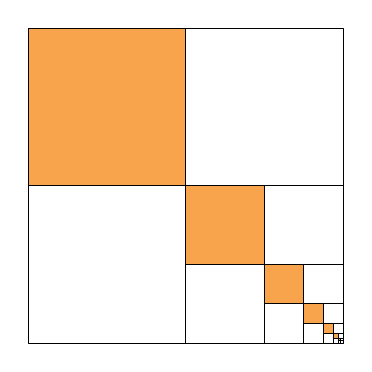
\begin{tikzpicture}[scale=1, main, line join=bevel]
		\fill[BurntOrange, nearly opaque] (2,2) -- (2,4) -- (0,4) -- (0,2) -- cycle;
		\fill[BurntOrange, nearly opaque] (2,2) -- (3,2) -- (3,1) -- (2,1) -- cycle;
		\fill[BurntOrange, nearly opaque] (3,1) -- (3.5,1) -- (3.5,0.5) -- (3,0.5) -- cycle;
		\fill[BurntOrange, nearly opaque] (3.5,0.5) -- (3.75,0.5) -- (3.75,0.25) -- (3.5,0.25) -- cycle;
		\fill[BurntOrange, nearly opaque] (3.75,0.25) -- (3.875,0.25) -- (3.875,0.125) -- (3.75,0.125) -- cycle;
		\fill[BurntOrange, nearly opaque] (3.875,0.125) -- (3.9375,0.125) -- (3.9375,0.0625) -- (3.875,0.0625) -- cycle;
		\fill[BurntOrange, nearly opaque] (3.9375,0.0625) -- (3.96875,0.0625) -- (3.96875,0.03125) -- (3.9375,0.03125) -- cycle;
		
		\draw[main] (0,0) -- (4,0) -- (4,4) -- (0,4) -- cycle;
		
		\draw[main] (2,0) -- (2,4);
		\draw[main] (0,2) -- (4,2);
		
		\draw[main] (2,1) -- (4,1);
		\draw[main] (3,0) -- (3,2);
		
		\draw[main] (3,0.5) -- (4,0.5);
		\draw[main] (3.5,0) -- (3.5,1);
		
		\draw[main] (3.5,0.25) -- (4,0.25);
		\draw[main] (3.75,0) -- (3.75,0.5);
		
		\draw[main] (3.75,0.125) -- (4,0.125);
		\draw[main] (3.875,0) -- (3.875,0.25);
		
		\draw[main] (3.875,0.0625) -- (4,0.0625);
		\draw[main] (3.9375,0) -- (3.9375,0.125);
		
		\draw[main] (3.9375,0.03125) -- (4,0.03125);
		\draw[main] (3.96875,0) -- (3.96875,0.0625);
	\end{tikzpicture}
	
	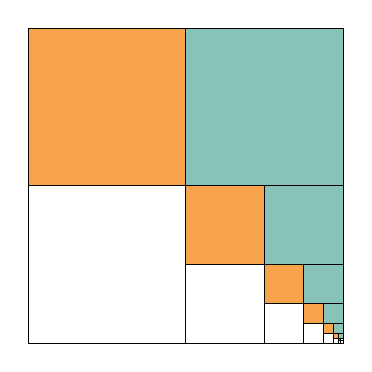
\begin{tikzpicture}[scale=1, main, line join=bevel]
		\fill[BurntOrange, nearly opaque] (2,2) -- (2,4) -- (0,4) -- (0,2) -- cycle;
		\fill[BurntOrange, nearly opaque] (2,2) -- (3,2) -- (3,1) -- (2,1) -- cycle;
		\fill[BurntOrange, nearly opaque] (3,1) -- (3.5,1) -- (3.5,0.5) -- (3,0.5) -- cycle;
		\fill[BurntOrange, nearly opaque] (3.5,0.5) -- (3.75,0.5) -- (3.75,0.25) -- (3.5,0.25) -- cycle;
		\fill[BurntOrange, nearly opaque] (3.75,0.25) -- (3.875,0.25) -- (3.875,0.125) -- (3.75,0.125) -- cycle;
		\fill[BurntOrange, nearly opaque] (3.875,0.125) -- (3.9375,0.125) -- (3.9375,0.0625) -- (3.875,0.0625) -- cycle;
		\fill[BurntOrange, nearly opaque] (3.9375,0.0625) -- (3.96875,0.0625) -- (3.96875,0.03125) -- (3.9375,0.03125) -- cycle;
		
		\fill[PineGreen, semitransparent] (2,2) -- (2,4) -- (4,4) -- (4,2) -- cycle;
		\fill[PineGreen, semitransparent] (3,1) -- (3,2) -- (4,2) -- (4,1) -- cycle;
		\fill[PineGreen, semitransparent] (3.5,0.5) -- (3.5,1) -- (4,1) -- (4,0.5) -- cycle;
		\fill[PineGreen, semitransparent] (3.75,0.25) -- (3.75,0.5) -- (4,0.5) -- (4,0.25) -- cycle;
		\fill[PineGreen, semitransparent] (3.875,0.125) -- (3.875,0.25) -- (4,0.25) -- (4,0.125) -- cycle;
		\fill[PineGreen, semitransparent] (3.9375,0.0625) -- (3.9375,0.125) -- (4,0.125) -- (4,0.0625) -- cycle;

		
		\draw[main] (0,0) -- (4,0) -- (4,4) -- (0,4) -- cycle;
		
		\draw[main] (2,0) -- (2,4);
		\draw[main] (0,2) -- (4,2);
		
		\draw[main] (2,1) -- (4,1);
		\draw[main] (3,0) -- (3,2);
		
		\draw[main] (3,0.5) -- (4,0.5);
		\draw[main] (3.5,0) -- (3.5,1);
		
		\draw[main] (3.5,0.25) -- (4,0.25);
		\draw[main] (3.75,0) -- (3.75,0.5);
		
		\draw[main] (3.75,0.125) -- (4,0.125);
		\draw[main] (3.875,0) -- (3.875,0.25);
		
		\draw[main] (3.875,0.0625) -- (4,0.0625);
		\draw[main] (3.9375,0) -- (3.9375,0.125);
		
		\draw[main] (3.9375,0.03125) -- (4,0.03125);
		\draw[main] (3.96875,0) -- (3.96875,0.0625);
	\end{tikzpicture}
	
	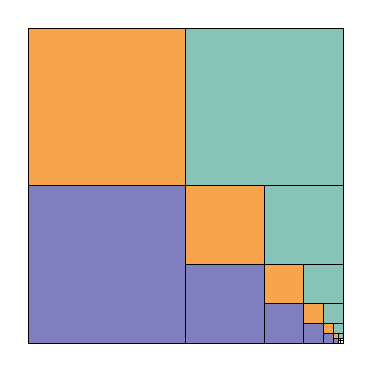
\begin{tikzpicture}[scale=1, main, line join=bevel]
		\fill[BurntOrange, nearly opaque] (2,2) -- (2,4) -- (0,4) -- (0,2) -- cycle;
		\fill[BurntOrange, nearly opaque] (2,2) -- (3,2) -- (3,1) -- (2,1) -- cycle;
		\fill[BurntOrange, nearly opaque] (3,1) -- (3.5,1) -- (3.5,0.5) -- (3,0.5) -- cycle;
		\fill[BurntOrange, nearly opaque] (3.5,0.5) -- (3.75,0.5) -- (3.75,0.25) -- (3.5,0.25) -- cycle;
		\fill[BurntOrange, nearly opaque] (3.75,0.25) -- (3.875,0.25) -- (3.875,0.125) -- (3.75,0.125) -- cycle;
		\fill[BurntOrange, nearly opaque] (3.875,0.125) -- (3.9375,0.125) -- (3.9375,0.0625) -- (3.875,0.0625) -- cycle;
		\fill[BurntOrange, nearly opaque] (3.9375,0.0625) -- (3.96875,0.0625) -- (3.96875,0.03125) -- (3.9375,0.03125) -- cycle;
		
		\fill[PineGreen, semitransparent] (2,2) -- (2,4) -- (4,4) -- (4,2) -- cycle;
		\fill[PineGreen, semitransparent] (3,1) -- (3,2) -- (4,2) -- (4,1) -- cycle;
		\fill[PineGreen, semitransparent] (3.5,0.5) -- (3.5,1) -- (4,1) -- (4,0.5) -- cycle;
		\fill[PineGreen, semitransparent] (3.75,0.25) -- (3.75,0.5) -- (4,0.5) -- (4,0.25) -- cycle;
		\fill[PineGreen, semitransparent] (3.875,0.125) -- (3.875,0.25) -- (4,0.25) -- (4,0.125) -- cycle;
		\fill[PineGreen, semitransparent] (3.9375,0.0625) -- (3.9375,0.125) -- (4,0.125) -- (4,0.0625) -- cycle;
		
		\fill[NavyBlue, semitransparent] (0,2) -- (2,2) -- (2,0) -- (0,0) -- cycle;
		\fill[NavyBlue, semitransparent] (2,1) -- (3,1) -- (3,0) -- (2,0) -- cycle;
		\fill[NavyBlue, semitransparent] (3,0.5) -- (3.5,0.5) -- (3.5,0) -- (3,0) -- cycle;
		\fill[NavyBlue, semitransparent] (3.5,0.25) -- (3.75,0.25) -- (3.75,0) -- (3.5,0) -- cycle;
		\fill[NavyBlue, semitransparent] (3.75,0.125) -- (3.875,0.125) -- (3.875,0) -- (3.75,0) -- cycle;
		\fill[NavyBlue, semitransparent] (3.875,0.0625) -- (3.9375,0.0625) -- (3.9375,0) -- (3.875,0) -- cycle;
		
		\draw[main] (0,0) -- (4,0) -- (4,4) -- (0,4) -- cycle;
		
		\draw[main] (2,0) -- (2,4);
		\draw[main] (0,2) -- (4,2);
		
		\draw[main] (2,1) -- (4,1);
		\draw[main] (3,0) -- (3,2);
		
		\draw[main] (3,0.5) -- (4,0.5);
		\draw[main] (3.5,0) -- (3.5,1);
		
		\draw[main] (3.5,0.25) -- (4,0.25);
		\draw[main] (3.75,0) -- (3.75,0.5);
		
		\draw[main] (3.75,0.125) -- (4,0.125);
		\draw[main] (3.875,0) -- (3.875,0.25);
		
		\draw[main] (3.875,0.0625) -- (4,0.0625);
		\draw[main] (3.9375,0) -- (3.9375,0.125);
		
		\draw[main] (3.9375,0.03125) -- (4,0.03125);
		\draw[main] (3.96875,0) -- (3.96875,0.0625);
	\end{tikzpicture}
\end{document}